\documentclass[11pt,a4paper]{article}
\usepackage[T1]{fontenc}
\usepackage{lmodern}
\usepackage[margin=2.4cm]{geometry}
\usepackage{booktabs,graphicx,amsmath,amssymb,float,caption,microtype}
\usepackage[table]{xcolor}
\usepackage[colorlinks=true,linkcolor=blue!55!black,urlcolor=blue!55!black,citecolor=blue!55!black]{hyperref}
\graphicspath{{../figures/}}
\captionsetup{font=small,labelfont=bf}
\setlength{\parskip}{0.4em}\setlength{\parindent}{0pt}
\setlength{\tabcolsep}{4.5pt}
\title{\textbf{Foreign-Exchange Volatility, Risk and Trend Strategies}\\[2pt]
\large A reproducible study of EUR/USD, GBP/USD and USD/JPY (2022--2024)}
\author{Dan Allouche}
\date{\today}
\begin{document}
\maketitle
\vspace{-1.2em}
\begin{abstract}
\noindent We ask one question of three FX majors over 2022--2024: \emph{does conditioning risk on
time-varying, fat-tailed volatility improve real risk decisions --- VaR/ES coverage and exception
independence --- or is a constant-variance model good enough?} We establish fat tails and clustering
(diagnostics), fit EWMA and GARCH(1,1) Student-$t$ volatility, and push the conditional volatility into
\textbf{conditional VaR/ES} (GARCH-filtered and Filtered Historical Simulation) backtested side-by-side
against the unconditional model (Kupiec, Christoffersen), validate the Expected Shortfall
(Acerbi--Székely) and model the regulatory tail by \textbf{Extreme Value Theory}, and finally let the vol
model \emph{size} a momentum strategy whose Sharpe carries bootstrap confidence intervals. The honest
finding: conditioning improves exception independence for the European pairs, while for USD/JPY parsimony
is hard to beat and the GARCH-$t$ ES is rejected. A methodological cornerstone: weekend/holiday dates are
\emph{non-observations}, not missing data --- a naive calendar imputation fabricates roughly a quarter of
the sample, so the study runs on the native 781 trading days. Every number is produced by a unit-tested
Python package and reproduces from a committed snapshot.
\end{abstract}
\tableofcontents
\vspace{0.5em}

\section{Introduction}
Volatility is the central object of FX risk management: it drives position sizing, option pricing
and Value-at-Risk. This report takes three liquid currency pairs --- EUR/USD, GBP/USD and USD/JPY ---
and carries volatility from a descriptive rolling estimate through to a fitted conditional model, a
backtested risk measure, and an out-of-sample forecast evaluation. The guiding principles are
\emph{honest data}, \emph{tested computation}, and \emph{claims traceable to printed values}: every
figure and table below is generated by the accompanying \texttt{fxvol} package and reproduces offline
from a committed snapshot.
The study addresses four questions: (i) what are the distributional and time-series properties of
daily FX returns; (ii) does conditional-volatility modelling (GARCH) add value over simpler baselines;
(iii) are standard risk measures well calibrated; and (iv) does a simple trend rule survive realistic
transaction costs?
\section{Data and methodology}
\subsection{Data}
Daily OHLC quotes for the three pairs are retrieved from Yahoo Finance for 2022-01-03--2024-12-30 and stored as a
committed Parquet snapshot (as-of 2026-06-14) so the analysis is deterministic and network-free. Each pair has
781 trading observations.
\subsection{The weekend-imputation pitfall}
FX trades Monday--Friday; Saturday and Sunday are \emph{non-observations}, not gaps to be filled.
An earlier version of this project reindexed each series onto a full 365-day calendar and imputed the
missing weekend/holiday rows with a recursive five-day rolling mean. Because the recursion feeds its
own imputed values back in, it is a low-pass filter that \textbf{fabricated 312 of 1093 calendar rows
($\approx$28\%)}. This contaminates every return, volatility, RSI and distributional statistic, induces
artificial autocorrelation, and---critically---breaks the annualization, since $\sqrt{252}$ assumes 252
observations per year while a calendar series has $\approx$365. We therefore discard the calendar
reindex entirely and compute all statistics on the native trading-day index; a unit test guarantees no
weekend row can re-enter the data. Table~\ref{tab:integrity} reports the integrity check.
\begin{table}[H]\centering
\small
\caption{Data-integrity check after trading-day alignment.}\label{tab:integrity}
\begin{tabular}{lr}
\toprule
 & Value \\
\midrule
Trading rows / pair & 781 \\
Weekend rows & 0 \\
First date & 2022-01-03 \\
Last date & 2024-12-30 \\
Calendar days spanned & 1093 \\
\bottomrule
\end{tabular}
\end{table}
\subsection{Returns, volatility and indicators}
We use log returns $r_t=\ln(P_t/P_{t-1})$ (time-additive). Annualized rolling volatility over a
window of $n$ trading days is $\hat\sigma^{\text{ann}}_t=\sqrt{252}\,\operatorname{sd}(r_{t-n+1},\dots,r_t)$,
with the factor matched to the trading-day frequency. As a decay-weighted alternative we use the
RiskMetrics EWMA recursion $\sigma_t^2=(1-\lambda)\,r_t^2+\lambda\,\sigma_{t-1}^2$ with
$\lambda=0.94$. Trend and momentum are summarised by simple moving averages and Wilder's RSI
(recursive smoothing with $\alpha=1/14$), the canonical definition.
\begin{table}[H]\centering
\small
\caption{Daily log-return summary statistics (\%).}\label{tab:ret}
\begin{tabular}{lrrrrrrr}
\toprule
 & Mean & Std & Min & Q25 & Median & Q75 & Max \\
\midrule
EURUSD & -0.011 & 0.496 & -1.859 & -0.296 & -0.013 & 0.279 & 1.821 \\
GBPUSD & -0.009 & 0.581 & -4.232 & -0.309 & 0.004 & 0.293 & 3.031 \\
USDJPY & 0.04 & 0.666 & -3.796 & -0.284 & 0.086 & 0.392 & 2.503 \\
\bottomrule
\end{tabular}
\end{table}
USD/JPY carries the only positive average drift, reflecting its sustained 2022--2024 appreciation,
while GBP/USD exhibits the widest range (Table~\ref{tab:ret}), a footprint of the late-2022 UK
fiscal episode.
\subsection{Visual overview}
Figure~\ref{fig:dash} gives a per-pair overview: the closing price with its 20/50-day moving
averages, the annualized rolling volatility, the daily-return distribution, and Wilder's RSI.
\begin{figure}[p]\centering
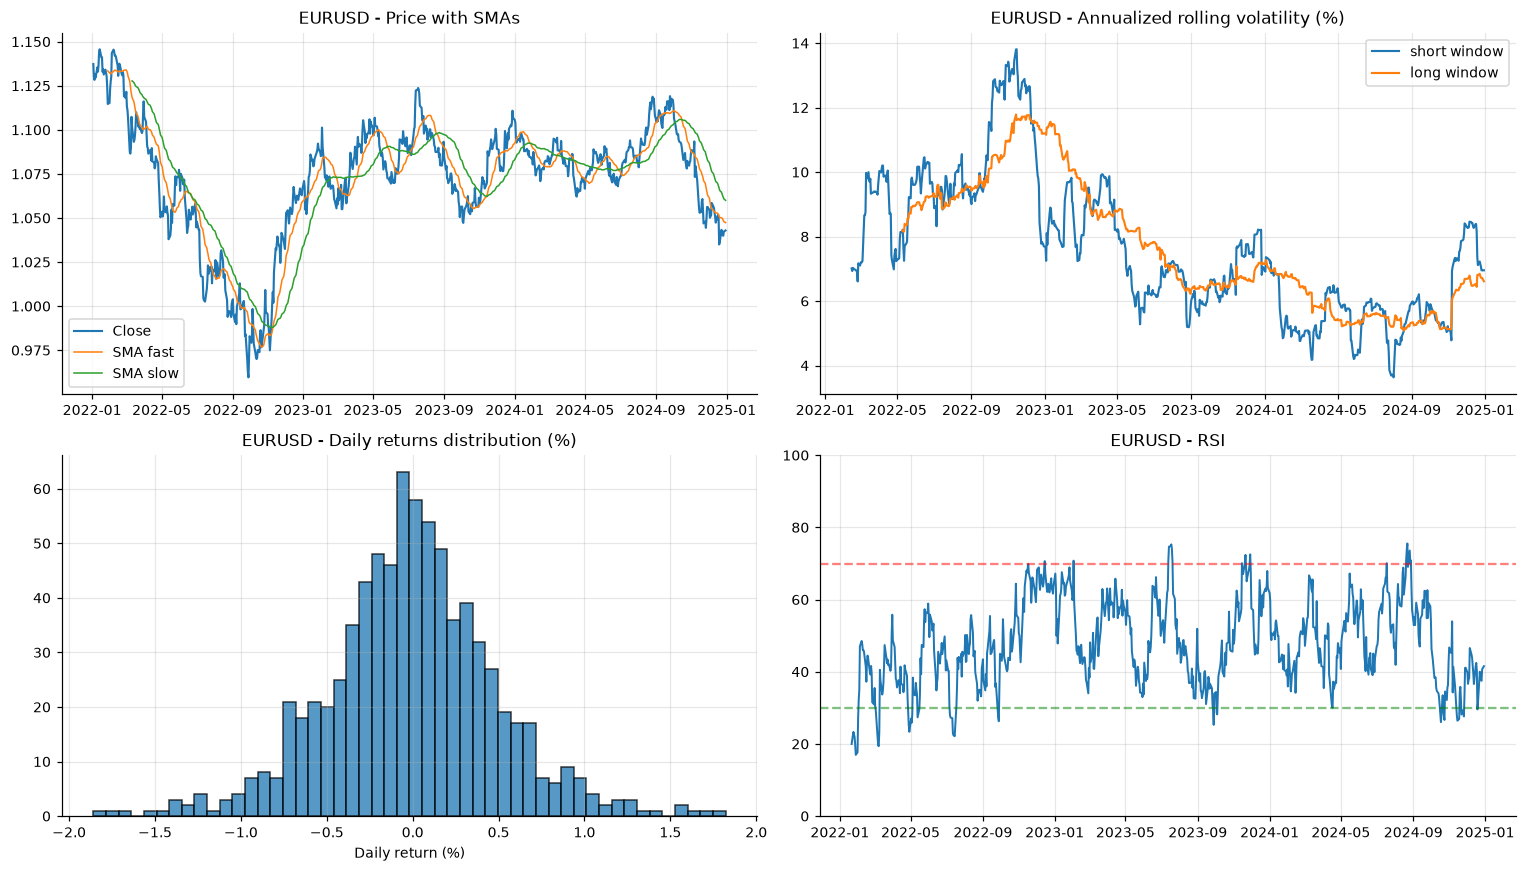
\includegraphics[width=0.74\linewidth,keepaspectratio]{dashboard_EURUSD.png}\\[3pt]
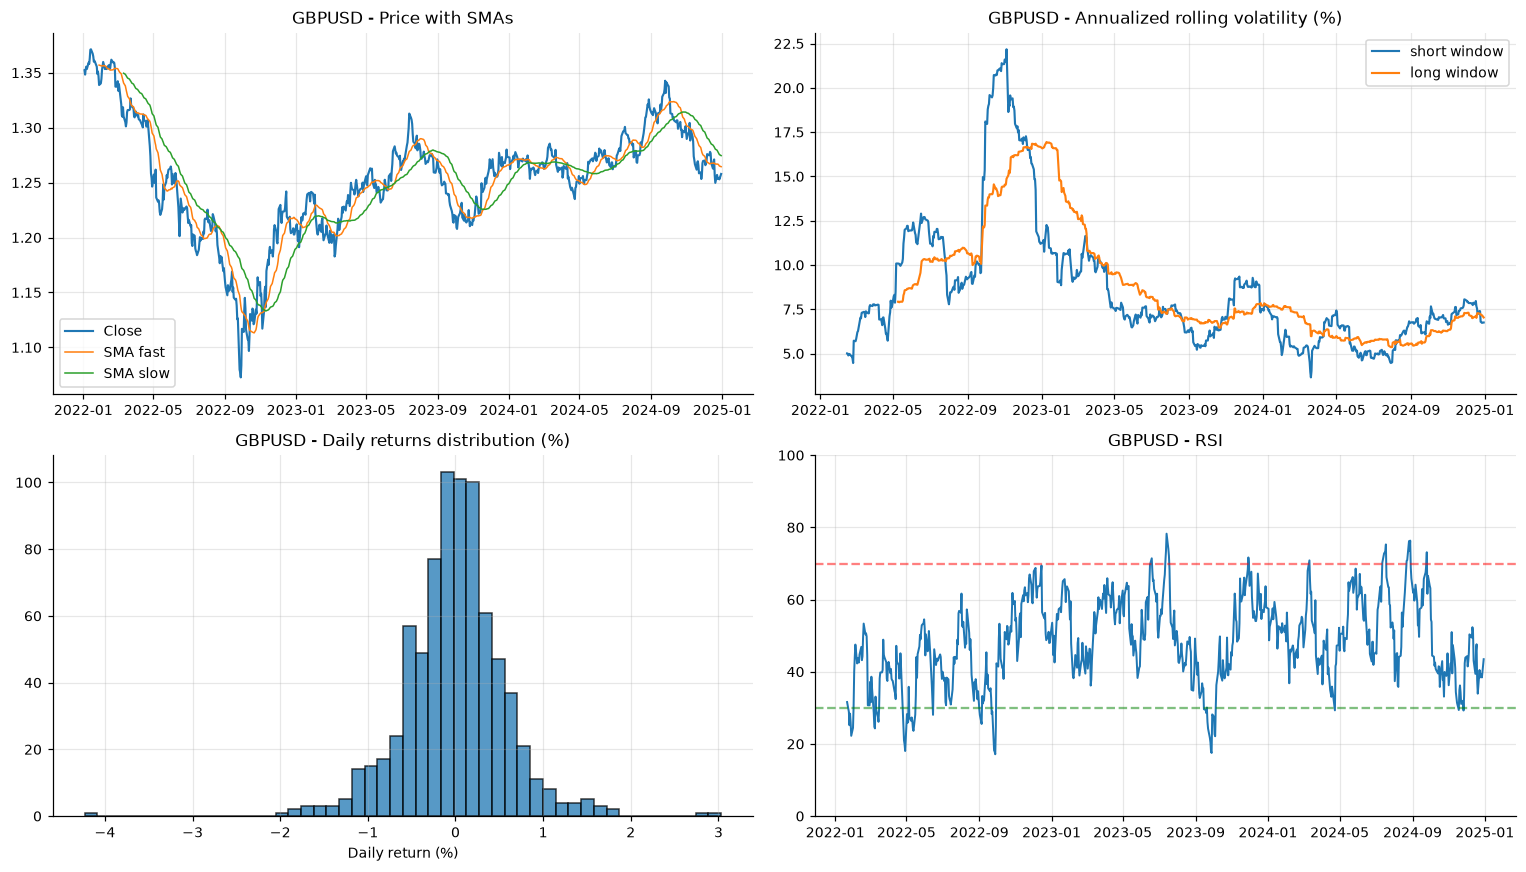
\includegraphics[width=0.74\linewidth,keepaspectratio]{dashboard_GBPUSD.png}\\[3pt]
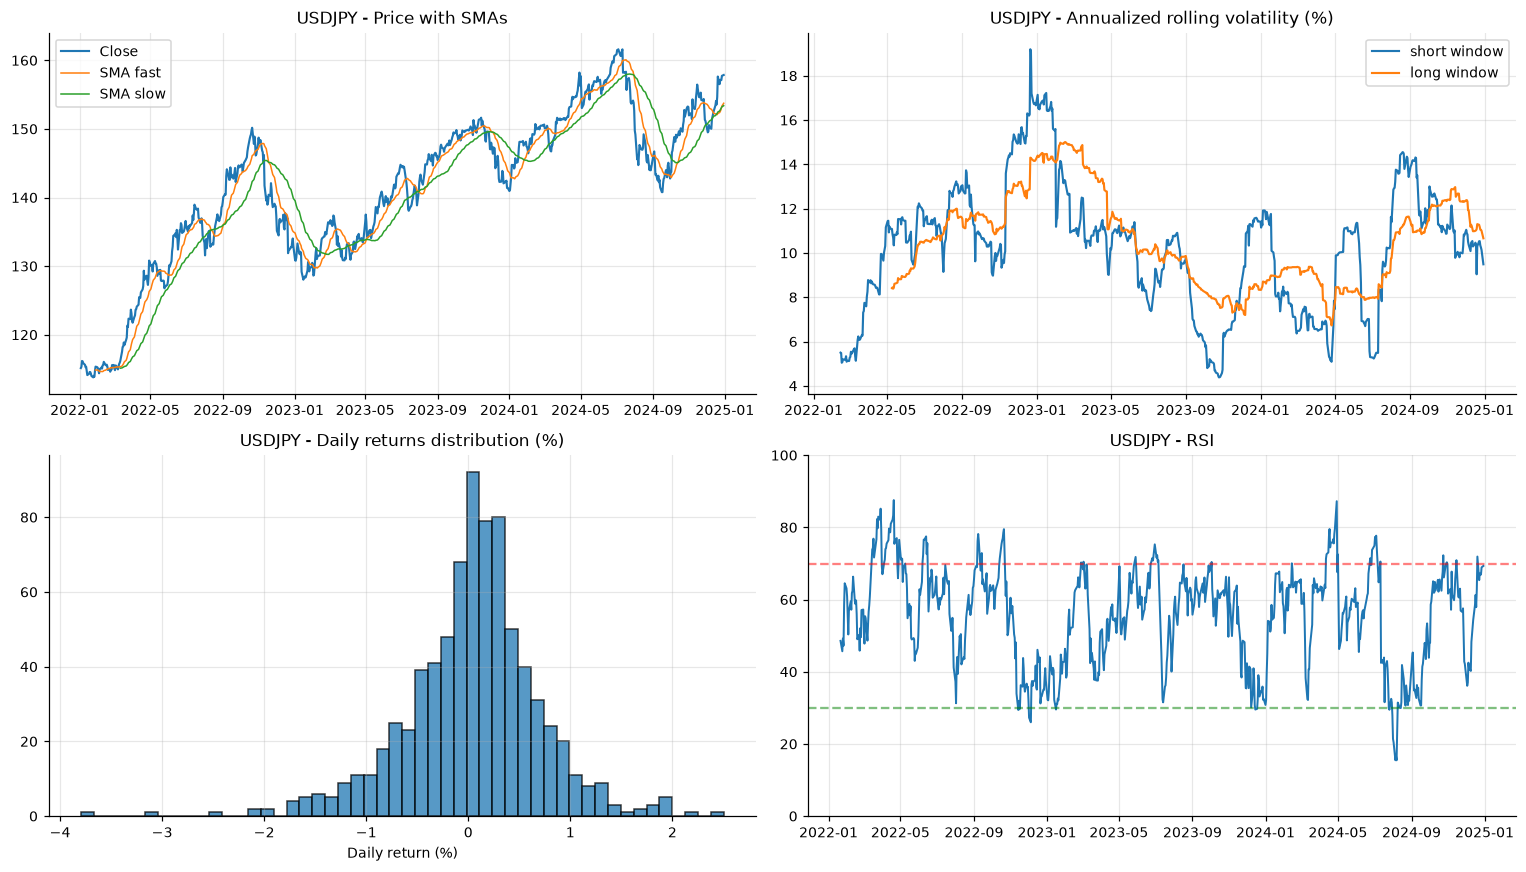
\includegraphics[width=0.74\linewidth,keepaspectratio]{dashboard_USDJPY.png}\\[3pt]
\caption{Per-pair dashboards: price with SMAs (top-left), annualized rolling volatility (top-right), daily-return histogram (bottom-left) and Wilder RSI (bottom-right).}\label{fig:dash}
\end{figure}
\section{Distributional and econometric diagnostics}
Before modelling we test the properties that justify the models. Table~\ref{tab:diag} reports skewness
and excess kurtosis, the Jarque--Bera (JB) normality test, ADF and KPSS stationarity tests, and
Ljung--Box (LB) and Engle ARCH-LM tests for autocorrelation and conditional heteroskedasticity.
\begin{table}[H]\centering
\small
\caption{Distributional and time-series diagnostics ($p$-values; LB at 10 lags).}\label{tab:diag}
\resizebox{\textwidth}{!}{%
\begin{tabular}{lrrrrrrrrr}
\toprule
 & Skew & Exc kurt & JB p & ADF ret p & KPSS ret p & LB ret p & LB sq p & ARCH-LM p & ADF price p \\
\midrule
EURUSD & -0.003 & 1.173 & $<$0.001 & $<$0.001 & 0.100 & 0.218 & $<$0.001 & $<$0.001 & 0.137 \\
GBPUSD & -0.265 & 5.543 & $<$0.001 & $<$0.001 & 0.100 & 0.151 & $<$0.001 & $<$0.001 & 0.143 \\
USDJPY & -0.516 & 2.823 & $<$0.001 & $<$0.001 & 0.100 & 0.599 & 0.427 & 0.576 & 0.284 \\
\bottomrule
\end{tabular}
}
\end{table}
Three facts emerge. (i) \textbf{Normality is rejected} for all pairs (JB $p<0.001$); returns are
leptokurtic, with excess kurtosis up to 5.5 for GBP/USD, visible in the QQ plot (Figure~\ref{fig:qq}).
(ii) Returns are \textbf{stationary} (ADF
rejects a unit root, KPSS does not), whereas log-prices are not---the standard $I(1)$ price / $I(0)$
return picture. (iii) \textbf{Volatility clustering} is present for the European pairs (squared-return
LB and ARCH-LM $p<0.001$), motivating GARCH; for USD/JPY the in-sample ARCH effect is weak
($p=0.58$), a nuance we carry through to the forecasting results.
\begin{figure}[H]\centering
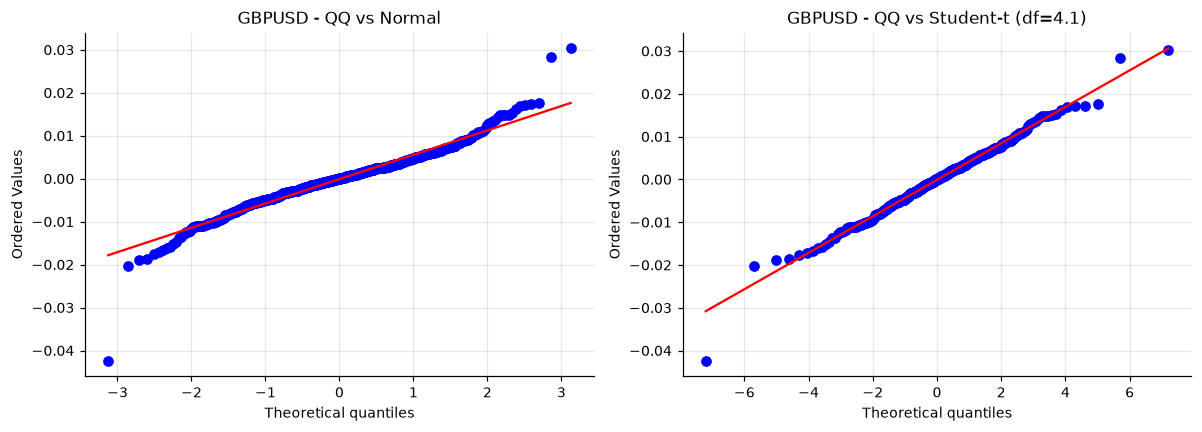
\includegraphics[width=0.92\linewidth,keepaspectratio]{qq_GBPUSD.png}
\caption{GBP/USD return quantiles against the Normal and a fitted Student-$t$. The heavy tails are evident in the departures from the Normal line.}\label{fig:qq}
\end{figure}
\section{Conditional-volatility modelling}
We fit a GARCH(1,1) with Student-$t$ innovations to each pair,
$\sigma_t^2=\omega+\alpha\,\epsilon_{t-1}^2+\beta\,\sigma_{t-1}^2$, where persistence is $\alpha+\beta$
and the unconditional (long-run) variance is $\omega/(1-\alpha-\beta)$. Table~\ref{tab:garch} reports
the estimates.
\begin{table}[H]\centering
\small
\caption{GARCH(1,1) Student-$t$ estimates (returns scaled $\times100$ for fitting).}\label{tab:garch}
\begin{tabular}{lrrrrrr}
\toprule
 & omega & alpha & beta & nu (dof) & persistence & Long-run vol (\%) \\
\midrule
EURUSD & 0.0006 & 0.0264 & 0.9715 & 7.7465 & 0.9979 & 8.6348 \\
GBPUSD & 0.0038 & 0.0488 & 0.9394 & 6.9151 & 0.9882 & 9.0531 \\
USDJPY & 0.0096 & 0.0723 & 0.9157 & 4.2933 & 0.988 & 14.1895 \\
\bottomrule
\end{tabular}
\end{table}
Persistence exceeds 0.98 for every pair---typical of daily FX, where volatility shocks decay slowly---
and the estimated degrees of freedom (4.3--7.7) confirm fat-tailed innovations. Figure~\ref{fig:cv}
overlays the GARCH conditional volatility on the rolling realized volatility and the EWMA estimate.
\begin{figure}[H]\centering
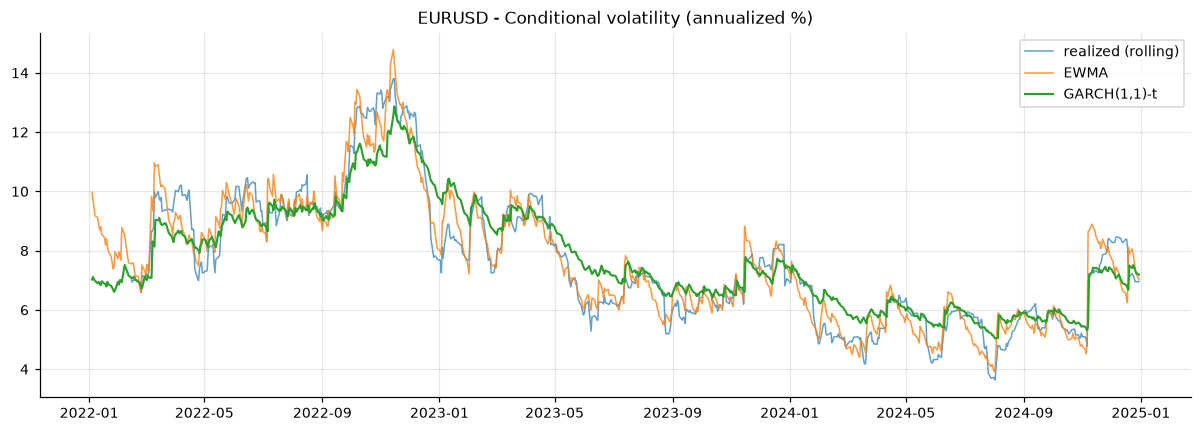
\includegraphics[width=0.92\linewidth,keepaspectratio]{cond_vol_EURUSD.png}\\[2pt]
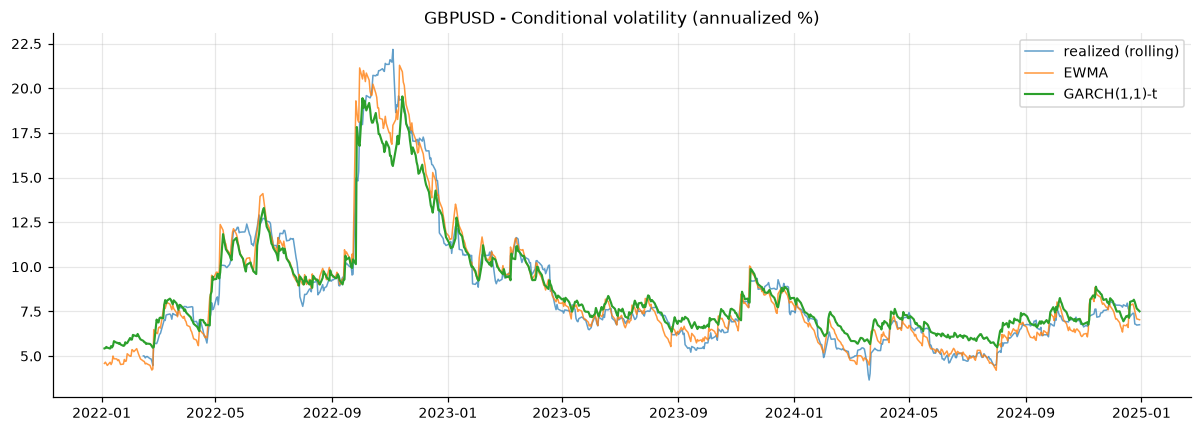
\includegraphics[width=0.92\linewidth,keepaspectratio]{cond_vol_GBPUSD.png}\\[2pt]
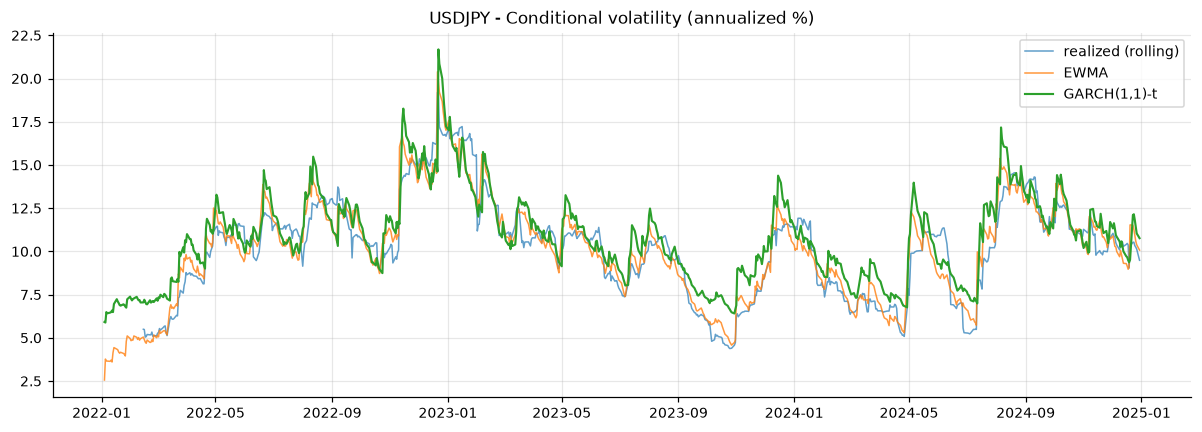
\includegraphics[width=0.92\linewidth,keepaspectratio]{cond_vol_USDJPY.png}\\[2pt]
\caption{Annualized conditional volatility (GARCH(1,1)-$t$), EWMA and rolling realized volatility.}\label{fig:cv}
\end{figure}
\section{Risk measurement}
For each pair we report one-day Value-at-Risk (VaR) and Expected Shortfall (ES) at the 95\% and
99\% levels, computed both historically and from a fitted Student-$t$, alongside annualized volatility,
Sharpe and Sortino ratios, and maximum drawdown (Tables~\ref{tab:risk1}--\ref{tab:risk2}). VaR/ES are
reported as positive loss fractions.
\begin{table}[H]\centering
\small
\caption{Risk summary: volatility, risk-adjusted return, drawdown and shape.}\label{tab:risk1}
\begin{tabular}{lrrrrrrr}
\toprule
 & Ann vol & Sharpe & Sortino & Max DD & DD dur & Skew & Exc kurt \\
\midrule
EURUSD & 0.0788 & -0.3553 & -0.3543 & -0.1651 & 184 & -0.0031 & 1.1726 \\
GBPUSD & 0.0922 & -0.2534 & -0.2446 & -0.221 & 184 & -0.2653 & 5.543 \\
USDJPY & 0.1057 & 0.965 & 0.8804 & -0.1503 & 62 & -0.5155 & 2.8228 \\
\bottomrule
\end{tabular}
\end{table}
\begin{table}[H]\centering
\small
\caption{One-day VaR and Expected Shortfall (loss fraction). H = historical, t = Student-$t$.}\label{tab:risk2}
\begin{tabular}{lrrrrrrrr}
\toprule
 & VaR H 95 & ES H 95 & VaR t 95 & ES t 95 & VaR H 99 & ES H 99 & VaR t 99 & ES t 99 \\
\midrule
EURUSD & 0.0081 & 0.0112 & 0.0081 & 0.0112 & 0.0131 & 0.0156 & 0.013 & 0.0167 \\
GBPUSD & 0.0097 & 0.0135 & 0.0089 & 0.0133 & 0.0159 & 0.021 & 0.0155 & 0.0215 \\
USDJPY & 0.0109 & 0.0159 & 0.0097 & 0.0151 & 0.0174 & 0.0241 & 0.0178 & 0.0255 \\
\bottomrule
\end{tabular}
\end{table}
\subsection{VaR backtesting}
We roll a 250-day historical 99\% VaR and test the breach sequence with the Kupiec proportion-of-failures
test (unconditional coverage) and the Christoffersen test (conditional coverage). All three pass at the
5\% level (Table~\ref{tab:vbt}), though USD/JPY is the weakest --- 9 breaches vs 5.3 expected, Kupiec
$p=0.142$, Christoffersen $p=0.112$ --- foreshadowing the Expected-Shortfall rejection in \S\ref{sec:es}.
\begin{table}[H]\centering
\small
\caption{VaR backtest at 99\% (rolling 250-day historical VaR).}\label{tab:vbt}
\begin{tabular}{lrrrr}
\toprule
 & Breaches & Expected & Kupiec p & Christ. cc p \\
\midrule
EURUSD & 4 & 5.3 & 0.553 & 0.813 \\
GBPUSD & 6 & 5.3 & 0.765 & 0.893 \\
USDJPY & 9 & 5.3 & 0.142 & 0.112 \\
\bottomrule
\end{tabular}
\end{table}
\section{Cross-pair dependence}
Table~\ref{tab:corr} reports the return correlation matrix and Table~\ref{tab:pca} the principal-
component decomposition. EUR/USD and GBP/USD co-move strongly ($+0.78$) and both move opposite USD/JPY,
consistent with a dominant USD factor. The first principal component explains \textbf{70.7\%} of joint
variance, so diversification across these three majors is limited. Figure~\ref{fig:dep} shows the
correlation heatmap and the 60-day rolling correlations, which widen markedly in stress periods.
\begin{table}[H]\centering
\small
\caption{Return correlation matrix.}\label{tab:corr}
\begin{tabular}{lrrr}
\toprule
 & EURUSD & GBPUSD & USDJPY \\
\midrule
EURUSD & 1 & 0.779 & -0.435 \\
GBPUSD & 0.779 & 1 & -0.439 \\
USDJPY & -0.435 & -0.439 & 1 \\
\bottomrule
\end{tabular}
\end{table}
\begin{table}[H]\centering
\small
\caption{First principal-component loadings (common USD factor).}\label{tab:pca}
\begin{tabular}{lr}
\toprule
 & PC1 loading \\
\midrule
EURUSD & -0.619 \\
GBPUSD & -0.62 \\
USDJPY & 0.483 \\
\bottomrule
\end{tabular}
\end{table}
\begin{figure}[H]\centering
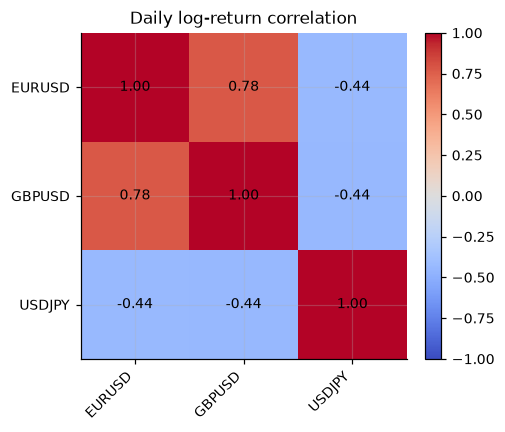
\includegraphics[width=0.46\linewidth,keepaspectratio]{corr_heatmap.png}\hfill
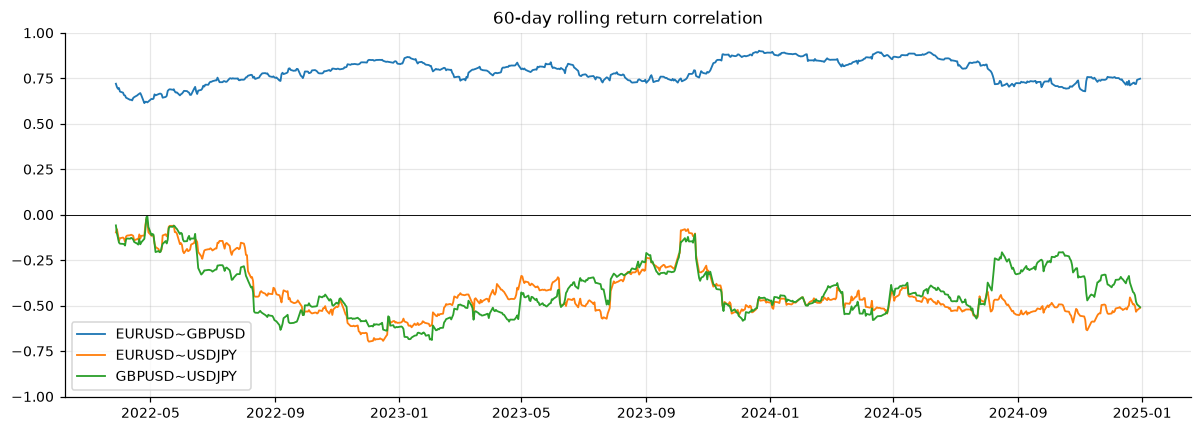
\includegraphics[width=0.52\linewidth,keepaspectratio]{rolling_corr.png}
\caption{Left: return correlation heatmap. Right: 60-day rolling correlations.}\label{fig:dep}
\end{figure}
\section{Trend strategy backtest}
We backtest a long/flat SMA(20/50) crossover. Signals are lagged one bar (next-bar execution, no
look-ahead), and a 1.0\,bp cost is charged on turnover. Performance is benchmarked against buy-and-hold
(Table~\ref{tab:bt}).
\begin{table}[H]\centering
\small
\caption{SMA crossover performance vs buy-and-hold (B\&H).}\label{tab:bt}
\resizebox{\textwidth}{!}{%
\begin{tabular}{lrrrrrrrrrr}
\toprule
 & Total ret & CAGR & Ann vol & Sharpe & Sortino & Max DD & Turnover & Hit rate & B\&H ret & B\&H Sharpe \\
\midrule
EURUSD & 0.0216 & 0.0069 & 0.045 & 0.1757 & 0.1303 & -0.0821 & 5.1692 & 0.4459 & -0.083 & -0.316 \\
GBPUSD & 0.05 & 0.0159 & 0.0549 & 0.3144 & 0.2176 & -0.0408 & 4.5231 & 0.5209 & -0.0698 & -0.2075 \\
USDJPY & 0.2572 & 0.0768 & 0.0812 & 0.9511 & 0.7347 & -0.0945 & 4.8462 & 0.5742 & 0.3711 & 1.0192 \\
\bottomrule
\end{tabular}
}
\end{table}
The rule improves the Sharpe ratio over buy-and-hold for \textbf{EURUSD, GBPUSD}---by stepping aside during the
2022--2023 downtrends where holding lost money---but it does \emph{not} beat USD/JPY's persistent uptrend
once costs are paid. We deliberately use a single textbook parameterization (no grid search), so in-sample
optimism is minimal. Figure~\ref{fig:eq} shows the equity curves.
\begin{figure}[H]\centering
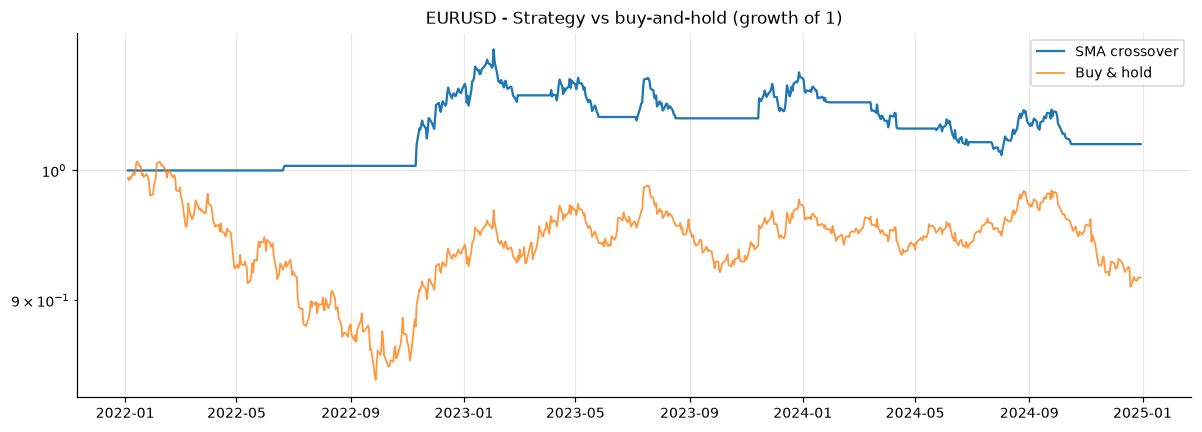
\includegraphics[width=0.80\linewidth,keepaspectratio]{equity_EURUSD.png}\\[2pt]
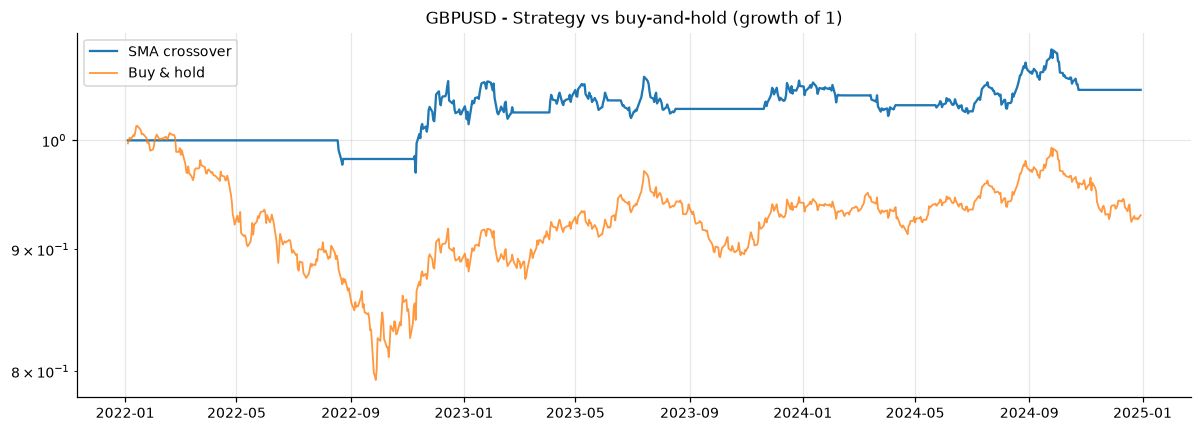
\includegraphics[width=0.80\linewidth,keepaspectratio]{equity_GBPUSD.png}\\[2pt]
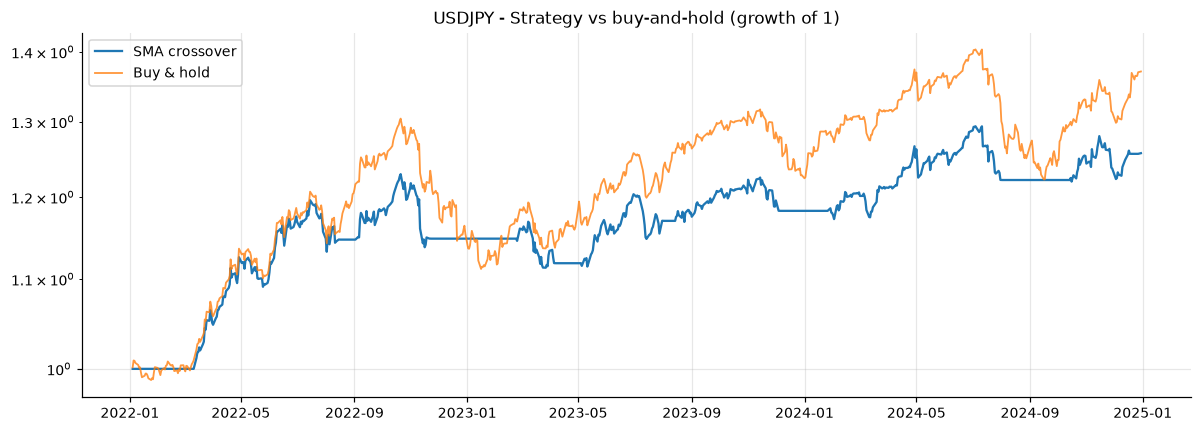
\includegraphics[width=0.80\linewidth,keepaspectratio]{equity_USDJPY.png}\\[2pt]
\caption{Strategy vs buy-and-hold growth of 1 (log scale).}\label{fig:eq}
\end{figure}
\section{Out-of-sample volatility forecasting}
Finally we ask whether conditional-volatility modelling pays off out-of-sample. Using an expanding
window, each model issues a one-day-ahead variance forecast; we score them with the QLIKE loss
$L(\sigma^2,\hat\sigma^2)=\sigma^2/\hat\sigma^2-\ln(\sigma^2/\hat\sigma^2)-1$ against the squared-return
proxy, and test differences with the Diebold--Mariano (DM) statistic (negative $=$ GARCH better).
The ``naive'' benchmark is the expanding constant variance (Table~\ref{tab:hr}).
\begin{table}[H]\centering
\small
\caption{Out-of-sample mean QLIKE per model and DM test of GARCH vs the naive benchmark.}\label{tab:hr}
\begin{tabular}{lrrrrlrr}
\toprule
 & GARCH & EWMA & Rolling & Naive & Best & DM vs naive & p \\
\midrule
EURUSD & 1.57 & 1.606 & 1.721 & 1.665 & garch & -1.3 & 0.195 \\
GBPUSD & 1.565 & 1.556 & 1.637 & 1.769 & ewma & -4.46 & 0 \\
USDJPY & 1.98 & 1.995 & 2.208 & 1.915 & naive & 1.03 & 0.302 \\
\bottomrule
\end{tabular}
\end{table}
GARCH and EWMA beat the constant-variance benchmark on the European pairs (the DM difference is
significant at 5\% for GBPUSD). For \textbf{USD/JPY the naive benchmark wins}---consistent with its weak
in-sample ARCH effect (\S3): when conditional heteroskedasticity is faint, a constant-variance forecast
is hard to beat.
\section{Conditional vs unconditional risk --- the research spine}
We now answer the central question. The GARCH conditional volatility is pushed into a one-day
\textbf{conditional VaR/ES}: a GARCH-filtered parametric Student-$t$ and a Filtered Historical Simulation
(FHS) on standardized residuals. These are backtested against the rolling unconditional historical and
Student-$t$ VaR on identical out-of-sample dates. Table~\ref{tab:kup95} shows the 95\% Kupiec coverage
$p$-values: the unconditional Student-$t$ VaR is mis-calibrated (too few breaches), while the conditional
models are well calibrated. Table~\ref{tab:ind99} shows the Christoffersen \emph{independence} $p$-values
at 99\%: conditioning reduces the breach clustering that static VaR suffers in the 2022 stress.
\begin{table}[H]\centering
\small
\caption{Kupiec coverage $p$-values at 95\% VaR (rows: model, columns: pair).}\label{tab:kup95}
\begin{tabular}{lrrr}
\toprule
 & EURUSD & GBPUSD & USDJPY \\
\midrule
hist & 0.26 & 0.118 & 0.26 \\
t & 0.013 & 0.044 & 0.103 \\
garch\_t & 0.361 & 0.18 & 0.376 \\
fhs & 0.482 & 0.18 & 0.759 \\
\bottomrule
\end{tabular}
\end{table}
\begin{table}[H]\centering
\small
\caption{Christoffersen independence $p$-values at 99\% VaR (rows: model, columns: pair).}\label{tab:ind99}
\begin{tabular}{lrrr}
\toprule
 & EURUSD & GBPUSD & USDJPY \\
\midrule
hist & 0.805 & 0.71 & 0.118 \\
t & 0.853 & 0.853 & 0.599 \\
garch\_t & 0.805 & 0.853 & 0.195 \\
fhs & 0.805 & 0.902 & 0.291 \\
\bottomrule
\end{tabular}
\end{table}
\section{Expected Shortfall backtest and EVT tails}\label{sec:es}
ES --- not VaR --- is the FRTB/Basel measure, so we validate the same GARCH-filtered Student-$t$ ES
of \S9 with the Acerbi--Székely (2014) $Z_2$ test ($E[Z_2]=0$ under correct ES; $Z_2<0$ means tail risk is understated),
with a $p$-value simulated from the model's own predictive law (Table~\ref{tab:esbt}). The ES is accepted
for the European pairs but \textbf{rejected for USD/JPY} --- the conditional model understates its tail,
exactly the pair with weak in-sample ARCH. This motivates an Extreme-Value tail: a Generalized Pareto
(Peaks-Over-Threshold, McNeil--Frey) fit to the standardized-residual tail (Table~\ref{tab:evt}); the
positive shape $\xi$ confirms heavier-than-exponential tails the single Student-$t$ cannot fully capture.
\begin{table}[H]\centering
\small
\caption{Acerbi--Székely $Z_2$ ES backtest of the GARCH-filtered Student-$t$ model at 99\%.}\label{tab:esbt}
\begin{tabular}{lrrrr}
\toprule
 & Z2 & p-value & breaches & expected \\
\midrule
EURUSD & 0.101 & 0.555 & 4 & 5.3 \\
GBPUSD & 0.497 & 0.876 & 3 & 5.3 \\
USDJPY & -1.147 & 0.016 & 11 & 5.3 \\
\bottomrule
\end{tabular}
\end{table}
\begin{table}[H]\centering
\small
\caption{POT/GPD tail of GARCH-standardized residuals (standardized scale).}\label{tab:evt}
\begin{tabular}{lrrrr}
\toprule
 & shape xi & n\_exceed & POT VaR99 (std) & POT ES99 (std) \\
\midrule
EURUSD & 0.119 & 78 & 2.6 & 3.36 \\
GBPUSD & 0.074 & 78 & 2.86 & 3.69 \\
USDJPY & 0.063 & 78 & 2.71 & 3.47 \\
\bottomrule
\end{tabular}
\end{table}
\section{Strategy with error bars}
Finally the volatility model is put to work \emph{sizing} risk: a time-series-momentum signal scaled
to a 10\% annualized vol target via the EWMA forecast, compared with the SMA crossover. Crucially every
Sharpe is reported with a stationary-block-bootstrap 95\% confidence interval and a Probabilistic Sharpe
Ratio (Table~\ref{tab:ci}). On $\sim$750 daily observations \textbf{every bootstrap CI straddles zero,
including USD/JPY ($[-0.15, 2.08]$)} --- so no Sharpe is significant at 95\%; only USD/JPY reaches a
Probabilistic Sharpe Ratio above 0.95, and that rests on a single persistent trend.
\begin{table}[H]\centering
\small
\caption{Strategy Sharpe with bootstrap 95\% CI and Probabilistic Sharpe Ratio (PSR).}\label{tab:ci}
\begin{tabular}{lrrrr}
\toprule
pair / strategy & Sharpe & CI low & CI high & PSR \\
\midrule
EURUSD SMA(20/50) & 0.176 & -0.93 & 1.25 & 0.622 \\
EURUSD TSMOM vol-target & -0.103 & -1.13 & 0.91 & 0.429 \\
GBPUSD SMA(20/50) & 0.314 & -0.63 & 1.27 & 0.71 \\
GBPUSD TSMOM vol-target & 0.409 & -0.61 & 1.41 & 0.764 \\
USDJPY SMA(20/50) & 0.951 & -0.15 & 2.08 & 0.951 \\
USDJPY TSMOM vol-target & 0.956 & -0.16 & 2.05 & 0.953 \\
\bottomrule
\end{tabular}
\end{table}
Figure~\ref{fig:tsmom} shows the volatility-targeted equity curves.
\begin{figure}[H]\centering
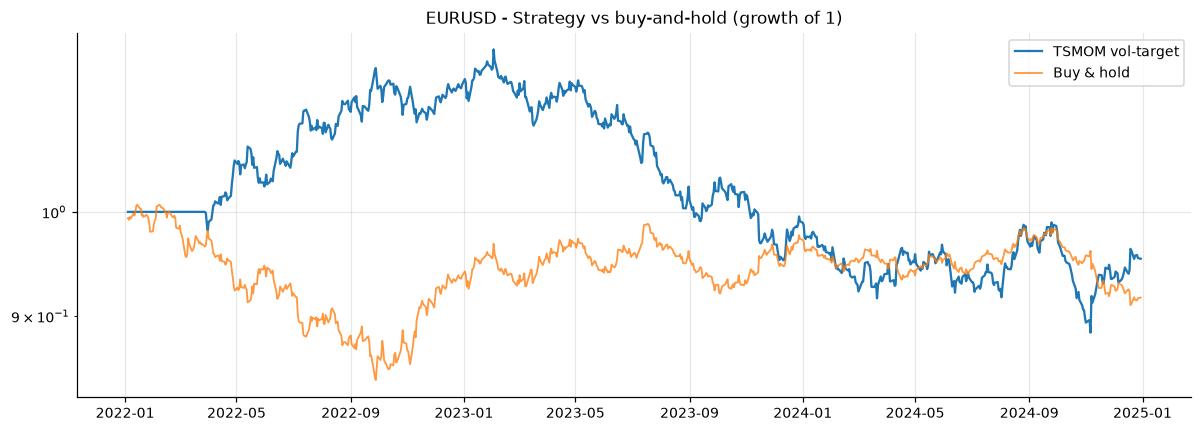
\includegraphics[width=0.78\linewidth,keepaspectratio]{equity_tsmom_EURUSD.png}\\[2pt]
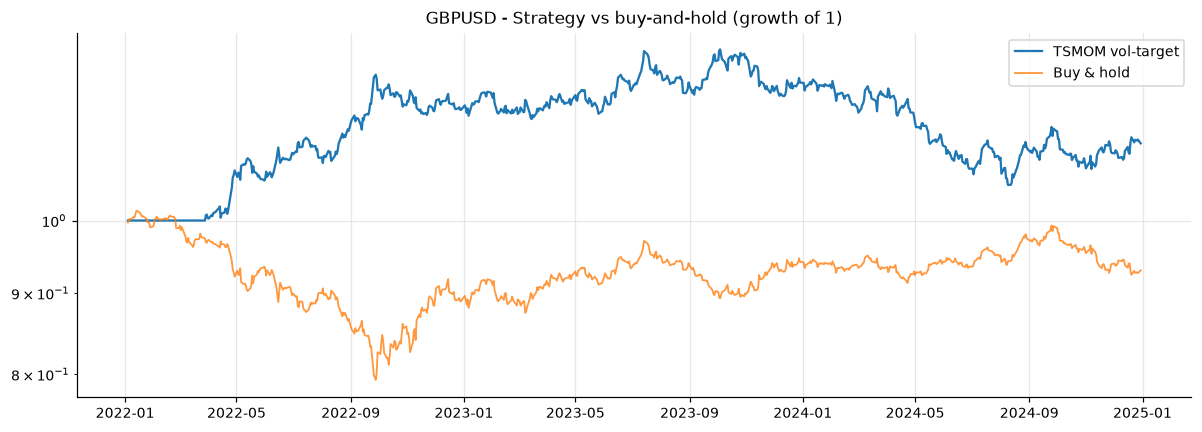
\includegraphics[width=0.78\linewidth,keepaspectratio]{equity_tsmom_GBPUSD.png}\\[2pt]
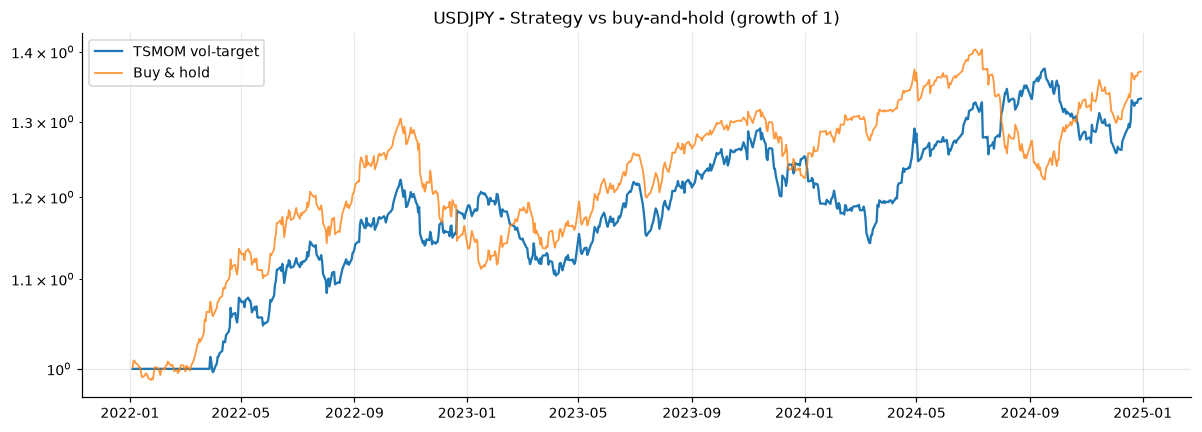
\includegraphics[width=0.78\linewidth,keepaspectratio]{equity_tsmom_USDJPY.png}\\[2pt]
\caption{Volatility-targeted TSMOM strategy vs buy-and-hold (growth of 1, log scale).}\label{fig:tsmom}
\end{figure}
\section{Discussion and limitations}
The results cohere into one answer: conditioning FX risk on time-varying, fat-tailed volatility
improves VaR exception \emph{independence} and gives well-calibrated ES \emph{where clustering is strong}
(the European pairs); where in-sample ARCH is weak (USD/JPY) the parsimonious model is competitive and the
GARCH-$t$ ES is even rejected, which the EVT tail addresses. Strategy edges, honestly error-barred, are
mostly indistinguishable from luck on this sample. Limitations: daily data over three years; a noisy
realized-variance proxy (mitigated by reporting range-based estimators); a single, deliberately
un-optimized strategy; and three pairs without asymmetric (GJR/EGARCH) or multivariate (DCC) volatility ---
deliberately scoped out as low signal-to-effort on this dataset. These are natural extensions.
\section{Conclusion}
On honest, weekend-free data, conditional-volatility modelling and properly backtested risk measures
add demonstrable value, while a simple trend strategy is regime-dependent once costs are paid. Every
number in this report is computed by tested code and reproduces from a committed snapshot via
\texttt{make setup \&\& make test \&\& make run}; the source, tests and notebook accompany this document.
\appendix
\section{Software and reproducibility}
The analysis is implemented in the \texttt{fxvol} Python package, organised into focused modules:
\texttt{data} (snapshot load / live refresh), \texttt{preprocessing} (trading-day alignment),
\texttt{indicators} (returns, rolling and EWMA volatility, SMA, RSI), \texttt{risk} (VaR/ES, drawdown,
Sharpe/Sortino, Kupiec/Christoffersen), \texttt{models} (EWMA, GARCH, walk-forward forecasting, QLIKE,
Diebold--Mariano), \texttt{diagnostics} (JB, ADF, KPSS, Ljung--Box, ARCH-LM), \texttt{backtest}, and
\texttt{plots}. The notebook is a thin narrative layer that imports this package.

A \texttt{pytest} suite of 60 tests guards correctness: indicator golden values (e.g.\ Cutler RSI against
a hand computation, the $\sqrt{252}$ annualization identity, the EWMA recursion), VaR/ES cross-checks
(historical vs Normal on Gaussian data, Student-$t \to$ Normal as the degrees of freedom grow, $ES>VaR$),
drawdown on a known path, Kupiec/Christoffersen calibration, a data-integrity check that no weekend row
can enter the series, and a no-look-ahead assertion on the backtest. Continuous integration runs the
linter, the test suite, and a headless execution of the notebook against the committed snapshot on every
push. The full study reproduces offline with:
\begin{quote}\texttt{make setup \&\& make test \&\& make run}\end{quote}
All inputs come from the committed Parquet snapshot; no network access is required to regenerate any
number, table or figure in this report.
\begin{thebibliography}{9}
\bibitem{wilder} J.~W.~Wilder. \emph{New Concepts in Technical Trading Systems}. Trend Research, 1978.
\bibitem{engle} R.~F.~Engle. Autoregressive conditional heteroscedasticity. \emph{Econometrica}, 50(4):987--1007, 1982.
\bibitem{bollerslev} T.~Bollerslev. Generalized autoregressive conditional heteroskedasticity. \emph{J.~Econometrics}, 31(3):307--327, 1986.
\bibitem{riskmetrics} J.P.~Morgan/Reuters. \emph{RiskMetrics Technical Document}, 4th ed., 1996.
\bibitem{kupiec} P.~Kupiec. Techniques for verifying the accuracy of risk measurement models. \emph{J.~Derivatives}, 3(2):73--84, 1995.
\bibitem{christoffersen} P.~Christoffersen. Evaluating interval forecasts. \emph{Int.~Econ.~Review}, 39(4):841--862, 1998.
\bibitem{dm} F.~X.~Diebold and R.~S.~Mariano. Comparing predictive accuracy. \emph{J.~Bus.~Econ.~Stat.}, 13(3):253--263, 1995.
\bibitem{patton} A.~J.~Patton. Volatility forecast comparison using imperfect volatility proxies. \emph{J.~Econometrics}, 160(1):246--256, 2011.
\end{thebibliography}
\end{document}